\documentclass[10pt]{article}
\usepackage[margin=0.7in]{geometry}
\usepackage{graphicx}
\begin{document}
\section*{Independent GLV held-out raw-row audit}
\textbf{2026-11-07.} Two content-addressed compressed row files matched their committed SHA-256 digests. An independent parser read 80,000 paired rows per arm, checked the full 2-family by 8-size by 200-curve by 25-target grid, and found 45,700 equal-table controls with zero count mismatches. All 16 cell point ratios and both primary geometric means match the published result to $10^{-15}$ absolute tolerance.
\medskip
\begin{center}\begin{tabular}{l|r|c|c}Family & Geometric mean & Independent 97.5\% interval & Published interval\\\hline $j=1728$ & 0.9565397206 & [0.948088, 0.964908] & [0.948003, 0.964895]\\$j=0$ & 0.9670782595 & [0.958173, 0.976202] & [0.958117, 0.976189]\end{tabular}\end{center}
\noindent The independent intervals use 10,000 curve-level resamples with a new seed. Endpoint differences are Monte Carlo variation; both upper bounds remain below one. The first PR commit \texttt{f630cc30} carried protocol, launcher, frozen analysis, and source before result commit \texttt{d433d5f9}. The commit order does not itself prove the first trial start time.
\begin{center}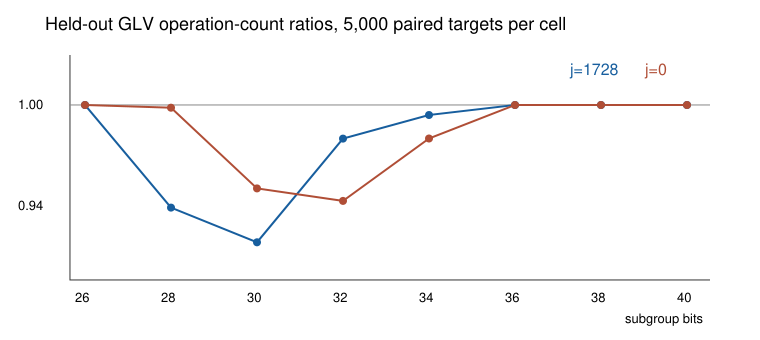
\includegraphics[width=0.95\linewidth]{cell-ratios.png}\end{center}
\noindent \textbf{Scope.} Operation-count ratios were recomputed from producer rows; correctness flags were only inspected. No native binary with the pinned digest was replayed, so the flags and counters lack an independent execution check. This run has no \texttt{experiment.export/v1} bundle, and no A/A arm was specified. The complete method, source hashes, and cell totals are in \texttt{REVIEW.md} and the adjacent scripts and JSON.
\end{document}
